\chapter{Maintenance}

This chapter explains how to maintain the catalog and Janitor itself. 
In order to administrate the catalog, it is absolutly recommened (but not required) to use the ontology editor Prot\`eg\`e. The first
section will explain how this is done.
The second section a detailed explanation how to create new packages for Janitor will be given.
In the last section typical use case in maintaining Janitor will be listed.

% * Maintainance
% ** Protege and RDF files
% ** Creating own tar balls

\section{Catalog}\label{sec:catalog}



The Catalog describes runtime environments and is either served through a web server or distributed together with the Janitor. 
It is specifed by a (Resource Description Framework) RDF file assigned to 
Janitor using the tag \texttt{catlog} within the configuration file (see~\ref{sec:janitor_configuration}). 
The format of the RDF file is defined by a RDF schema file \texttt{knowarc.rdfs}
which can be found along with an RDF example file \texttt{knowarc.rdf} in the janitor source directory \href{http://svn.nordugrid.org/repos/nordugrid/arc1/trunk/src/services/janitor/resources/catalog/}
{http://svn.nordugrid.org/repos/nordugrid/arc1/trunk/src/services/janitor/resources/catalog/}.\\


In order to adminstrate the catalog, the ontology editor Prot\`eg\`e should be used. Figure~\ref{fig:protege_example} shows the
editor while the MetaPackage \texttt{APPS/BIO/JASPAR-CORE-1.0} of the example file has been selected.
\begin{figure}
  \begin{center}
    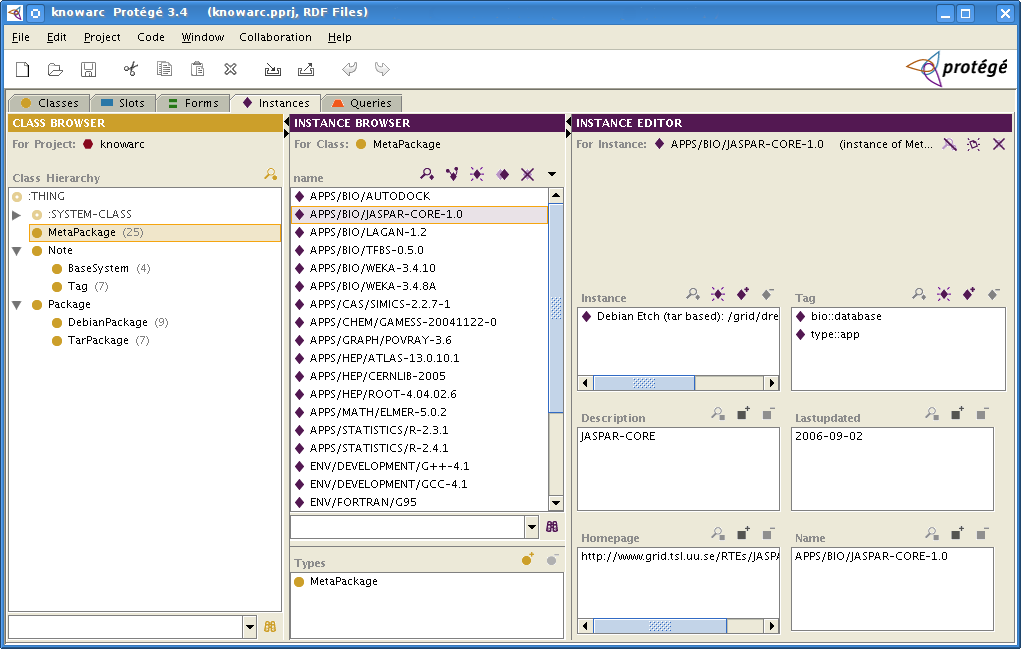
\includegraphics[width=\textwidth]{images/protege_JASPAR.png}
    \mycaption{Example of a RDF catalog file as displayed in the program Prot\`eg\`e.}{}
    \label{fig:protege_example}
  \end{center}
\end{figure}
On the left side of the editor the class browser is placed. Three main classes are prepared: \texttt{MetaPackage}, \texttt{Note} and \texttt{Package}.
The \texttt{Metapackage} is a general platform independent description of a \texttt{Package}. 
It has one or more instances of the class \texttt{Package} and is
described by the subclasses of \texttt{Note}. The class \texttt{Note} has two subclasses: \texttt{BaseSystem} 
and \texttt{Tag} to describe the \texttt{MetaPackage}. The \texttt{BaseSystem} describes the Debian release a \texttt{Package} refers to
(i.e. here etch or sid). The class \texttt{Tag} provides small keywords which can be assigned to \texttt{MetaPackages} such that
they can be easier found.  \texttt{TarPackage} and \texttt{DebianPackage} or currently the only subclasses of \texttt{Package}.
They are representing the necessary information (i.e. URL or Packagename) for the installation. In order to have an overview how the 
classes are interacting with each other the Tables~\ref{tab:main_class_meta},\ref{tab:main_class_base}, \ref{tab:main_class_tag},
\ref{tab:main_class_debian} and \ref{tab:main_class_tar} are pictured.

\begin{table}[!h]
   \begin{center}
        \mycaption{Specification of the class Metapackage.}{}
         \label{tab:main_class_meta}
	\begin{tabular}{p{3cm}p{3cm}p{4cm}}
	\textbf{Name}  & \textbf{Cardinality}  & \textbf{Type}\\
	\hline
	description    & single                & String       \\
	homepage       & single                & String       \\
	instance       & multiple              & Instance of Package       \\
	lastupdated    & single                & String       \\
	name           & required single       & String       \\
	tag            & multiple              & Instance of Tag       \\
	\end{tabular} 
   \end{center}
\end{table}


\begin{table}[!h]
   \begin{center}
        \mycaption{Specification of the class Basesystem.}{}
         \label{tab:main_class_base}
	\begin{tabular}{p{3cm}p{3cm}p{4cm}}
	\textbf{Name}  & \textbf{Cardinality}  & \textbf{Type}\\
	\hline
	description    & single                & String       \\
	distribution   & required single       & String       \\
	name           & required single       & String       \\
	short\_description & required single   & String       \\
	url            & required single       & String       \\
	\end{tabular} 
   \end{center}
\end{table}


\begin{table}[!h]
   \begin{center}
        \mycaption{Specification of the class Tag.}{}
         \label{tab:main_class_tag}
	\begin{tabular}{p{3cm}p{3cm}p{4cm}}
	\textbf{Name}  & \textbf{Cardinality}  & \textbf{Type}\\
	\hline
	description    & single                & String       \\
	name           & required single       & String       \\
	\end{tabular} 
   \end{center}
\end{table}

\begin{table}[!h]
   \begin{center}
        \mycaption{Specification of the class DebianPackage.}{}
         \label{tab:main_class_debian}
	\begin{tabular}{p{3cm}p{3cm}p{6cm}}
	\textbf{Name}  & \textbf{Cardinality}  & \textbf{Type}\\
	\hline
	basesystem     & required single       & Instance of BaseSystem       \\
	debconf        & multiple              & String       \\
	depends        & multiple              & Instance of MetaPackage  or Package      \\
	package        & required multiple              & String      \\
	\end{tabular} 
   \end{center}
\end{table}

\begin{table}[!h]
   \begin{center}
        \mycaption{Specification of the class TarPackage.}{}
         \label{tab:main_class_tar}
	\begin{tabular}{p{3cm}p{3cm}p{6cm}}
	\textbf{Name}  & \textbf{Cardinality}  & \textbf{Type}\\
	\hline
	basesystem     & required single       & Instance of BaseSystem       \\
	depends        & multiple              & Instance of MetaPackage or Package      \\
	environ        & multiple              & String       \\
	url            & required multiple     & String      \\
	\end{tabular} 
   \end{center}
\end{table}

\section{HTML interface of the catalog}

The dynamic Runtime Environments stored in the catalog are presented on the aforementioned dedicated web
page\footnote{http://dre.knowarc.eu:8080/list.pl}. This site also links to both the formal Catalog in 
RDF syntax and an automated transformation to
HTML. The latter mimics the traditional site describing Runtime Environments in the Runtime Environment
Registry\footnote{http://gridrer.csc.fi/} in order to minimise issues with an eventual transition to the new system. 
That page collects descriptions for Runtime Environments to encourage human site administrators to install these.
This html page listing the manually or automatically installable RTEs is prepared by the script web/list.pl.
This script is meant to be run by a mod-perl enabled Apache. The script itself is only loosely integrated
within the Janitor. In the first lines of the script some variables specific to the site are set. To configure the
script these have to be changed~\cite[p. 9]{BAYER_2007}.



\section{Introducing new packages}\label{sec:catalog}

This section describes how to add new packages to the catalog. Currently only tar based packages are processable by Janitor.
Within the example they are assigned to be used together with Debian Etch. This limitation is only literal. 
There should be no limitiation
to newer Debian distributions.

\subsection{Debian Etch (tar based)}

At the time of writing, only the tape archive (tar) file format is accepted for dynamic runtime environment installation, 
a well accepted file format throughout the UNIX community. This section explains the inner structure of the tar files. 
Subdirectories are visualised in Figure~\ref{fig:tar_folder}.

\begin{figure}
  \begin{center}
    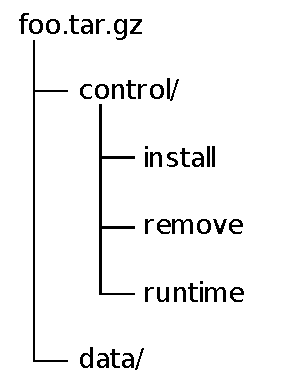
\includegraphics[width=4cm]{images/tar_folder.pdf}
    \mycaption{Directory structure in the tar files for automated installation.}{}
    \label{fig:tar_folder}
  \end{center}
\end{figure}

The tar file contains two directories named control and data. Software is stored in the latter subdirectory,
while the files formally specifying how to deal with such packages are stored in the prior. Upon installation,
the content of the data directory is extracted to some directory \textdollar BAR. 
After this unpacking of the tar file, the Janitor executes the install skript provided in the control directory. 
It is executed within the working directory \textdollar BAR. The job of this skript is to perform any necessary post-processing.
The Janitor stores the file \texttt{control/remove}. It will be executed in the same way as \texttt{control/install} just
before the tar-package is removed. In most cases \texttt{control/remove} will be empty.
Finally, the file \texttt{control/runtime} is sourced multiple times by the Grid Manager's job-submit script. After
installing the package, the Janitor changes all occurences of \%BASEDIR\% in the runtime script to \textdollar BAR.
To be offered to computing elements for an installation, the such prepared runtime environment must be
announced to a Catalog to which the Janitor on the computing element subscribes~\cite[p. 10]{BAYER_2007}.



\subsection{Protoypes}

In order to have an impression how the tar files are created, several prototypes are provided at \task{URL required!!}.:\\


The WEKA package for machine learning~\cite{FRANK_20074} and the Java Runtime Environment
are available as dynamic Runtime Environments. Further packages for bioinformatics comprise dynamic
variants of tools for the analysis of transcription factor binding sites. These are already offered for manual
installation via the prior mentioned traditional page representing Runtime Environments for ARC. 
The corresponding tar file is named \task{somewhat??}. The \texttt{data} directory simply contains a ZIP file
which needs to be unzipped in the installation directory. For that reason, the \texttt{control/install} script is 
written as follows:
% dollar signs made trouble in listings *hrmlgrmpf* ... Costs too much time to figure out why *ARC!*
\begin{verbatim} 
#!/bin/sh
set -e  # Makes the script to terminate at the first line it fails.

WEKA_ZIP="weka-3-4-8a.zip"
unzip $WEKA_ZIP
rm -f $WEKA_ZIP
\end{verbatim}
The runtime script sets the environment variable of the Java Classpath:
\begin{verbatim}
#!/bin/sh

WEKA_JAR="weka-3-4-8a/weka.jar"
case "\$1" in
	0)	# Just before job submission
		# none
	;;
	1)	# Just before job execution
		# Initialize the java environment
		CLASSPATH="%BASEDIR%/$WEKA_JAR:$CLASSPATH"
		export CLASSPATH
	;;
	2)	# After job termination
		# none
	;;
	*)
		return 1
	;;
esac	
\end{verbatim}
The remove script, which will be executed right before WEKA is deinstalled, is empty. Janitor will delete the directory, so there
is nothing to be done.\\



\textbf{CRAN and BioConductor.org} To demonstrate the technical proximity to scientific communities that
provide packages for the Debian Linux distribution, a tool was prepared to transform Debian packages to
dynamic runtime environments\cite{MOELLER_2007}. This effort comprising more than 1700 packages and
thus also helps to analyse the scalability of the RDF-based tool for the analysis of dependencies between
projects.  \task{Why is CRAN and BioConductor.org mentioned here??}\\


To address the concerns of the physicists using ARC, a dynamic runtime environment for the
ATLAS software suite was prepared. It extends prior work on an automated installation that is available at
\href{http://guts.uio.no/atlas/12.0.6/}{http://guts.uio.no/atlas/12.0.6/}. The preparation comprised the following steps:
\begin{itemize}
    \item The file system path specifications in the automated installation scripts were modified using the Janitor
       path variables.
    \item A tarball was prepared containing a directory structure as illustrated in Figure~\ref{fig:tar_folder}. The data directory
       was empty, since the automatic installation script downloads the software from a remote server.
    \item An entry was added to the Catalog file.
\end{itemize}
What sets High Energy Physics software apart is it's sheer size. The package in question takes up more than
5 GB. This was a test illustrating the feasibility of using DREs in High Energy Physics. The application
of the DRE for ATLAS needs to wait for the planned web service extension of the Catalog. With such a
service, e.g. a software manager of a big experiment will be able to deploy software packages on production
sites simply by creating a tarball and adding an entry to the Catalog.


\subsection{Debian Etch}

These kind of packages are not yet supported.

\subsection{Debian Sid}

These kind of packages are not yet supported.

\subsection{Adminstrating the Catalog}

\section{Typical use cases}\label{sec:catalog}

% ** setstate REMOVAL_PENDING
% no warranty interferences in the file syste,
